\documentclass[tikz,border=10pt]{standalone}
\usetikzlibrary{intersections}

\begin{document}
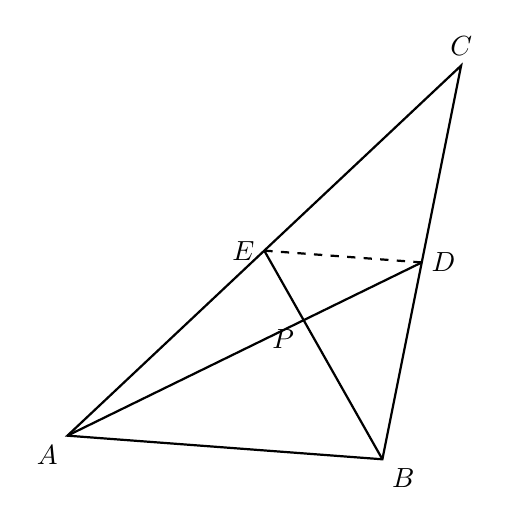
\begin{tikzpicture}
    % 1. 定义顶点坐标
    \coordinate (A) at (0,0.3);
    \coordinate (B) at (4,0);
    \coordinate (C) at (5,5);

    % 2. 定义边上的点 E 和 D
    % 使用比例来定点，便于调整位置
    \coordinate (E) at (barycentric cs:A=0.5,C=0.5); 
    \coordinate (D) at (barycentric cs:B=0.5,C=0.5);

    % 3. 绘制三角形主体
    \draw[thick] (A) -- (B) -- (C) -- cycle;

    % 4. 绘制内部线段 AD 和 BE
    \draw[thick, name path=AD] (A) -- (D);
    \draw[thick, name path=BE] (B) -- (E);

    % 5. 计算交点 P
    \path [name intersections={of=AD and BE, by=P}];

    % 6. 绘制辅助线 ED（虚线）
    \draw[dashed, thick] (E) -- (D);

    % 7. 标注点
    \node[below left] at (A) {$A$};
    \node[below right] at (B) {$B$};
    \node[above] at (C) {$C$};
    \node[left] at (E) {$E$};
    \node[right] at (D) {$D$};
    \node[below left] at (P) {$P$};

\end{tikzpicture}
\end{document}